\section{Ore di investimento}\label{oreInvestimento}
Le seguenti informazioni sono riportate solo a scopo informativo e \uline{non riguardano} il preventivo finale proposto al \gloxy{committente}.
\subsection{Dettaglio fasi non rendicontate}
\subsubsection{Fase di \fAt}
\subsubsubsection{Suddivisione del lavoro}
Nella fase di \fA, ciascun componente dovrà rivestire i seguenti ruoli:
%tabella suddivisione
\begin{table}[h]
\begin{center}
\begin{tabular}{|c|c|c|c|c|c|c|c|}
\hline Nome & Re & Am & An & Pt & Pr & Ve & Ore totali\\
\hline
\gma & 18 & 8 & - & - & - & 4 & 30 \\
\ao & - & 8 & 22 & - & - & - & 30 \\
\mb & - & 18 & 12 & - & - & - & 30 \\
\dm & 6 & 4 & 12 & - & - & 6 & 28 \\
\gmi & - & - & 20 & - & - & 7 & 27 \\
\sm & - & - & 23 & - & - & 5 & 28 \\
\fv & 6 & - & 12 & - & - & 11 & 29 \\
\hline Totale ruoli & 30 & 38 & 101 & - & - & 33 & 202 \\
\hline
\end{tabular}
\caption{Ore per ruolo - Fase di \fAt}
\end{center}
\end{table}
\FloatBarrier
I valori vengono riassunti nel seguente grafico:
%grafico suddivisione
\begin{figure}[htbp]
\centering
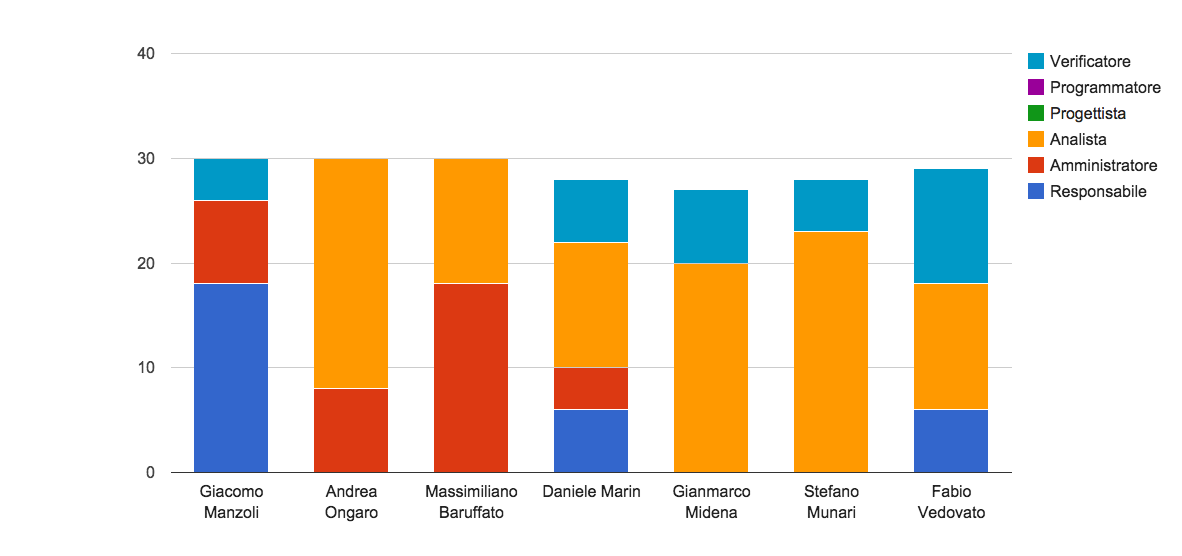
\includegraphics[width=\textwidth]{../immagini/nuoviGrafici/componenti/oreCompFaseAnalisi.png}
\caption{Ore per componente - Fase di \fAt}
\end{figure}
\FloatBarrier
\subsubsubsection{Prospetto economico}
Il totale delle ore di lavoro di ogni ruolo e il relativo costo \uline{a carico del \gloxy{fornitore}} vengono riportati nella seguente tabella:
%tabella costi
\begin{table}[h]
\begin{center}
\begin{tabular}{|m{3cm}|m{1.5cm}|m{1.5cm}|}
\hline Ruolo & Ore & Costo (\euro) \\
\hline
\rRPt & 30 & 900 \\
\rAPt & 38 & 950 \\
\rAt & 101 & 2222 \\
\rPt & 0 & 0 \\
\rpt & 0 & 0 \\
\rVt & 33 & 495 \\
\hline
Totale & 202 & 4567 \\
\hline
\end{tabular}
\caption{Costo per ruolo - Fase di \fAt}
\end{center}
\end{table}
\FloatBarrier
I seguenti grafici illustrano rispettivamente come ciascun ruolo abbia influito sul totale delle ore e dei costi \uline{a carico del \gloxy{fornitore}} durante la fase di \fA.
\begin{figure}[h]
\centering
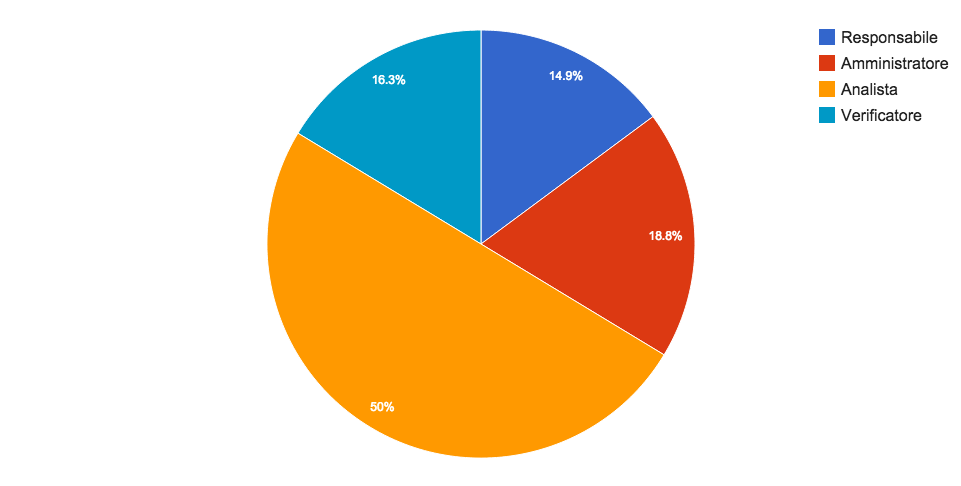
\includegraphics[width=0.9\textwidth]{../immagini/nuoviGrafici/oreFaseAnalisi.png}
\caption{Ore per ruoli - Fase di \fAt}
\end{figure}
\begin{figure}[h]
\centering
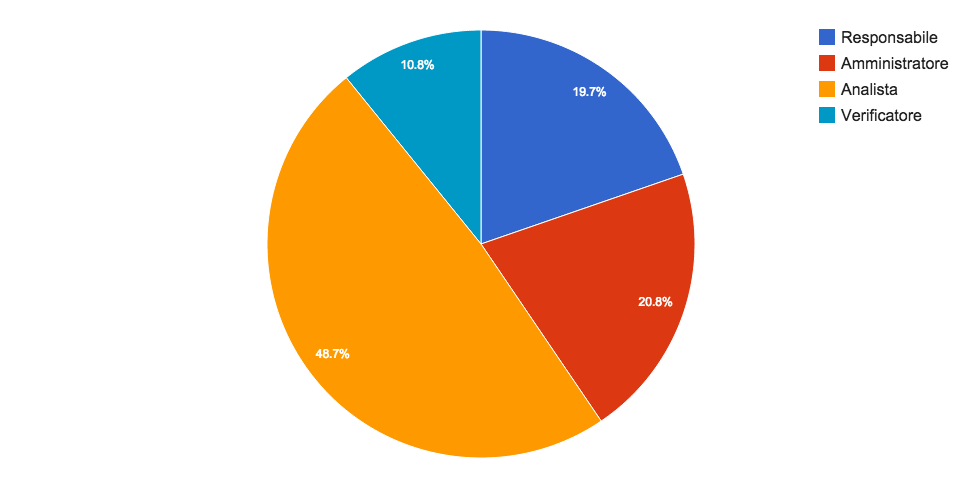
\includegraphics[width=0.9\textwidth]{../immagini/nuoviGrafici/costoFaseAnalisi.png}
\caption{Costi per ruoli - Fase di \fAt}
\end{figure}
\FloatBarrier
%\begin{figure}[htbp]
%\centering
%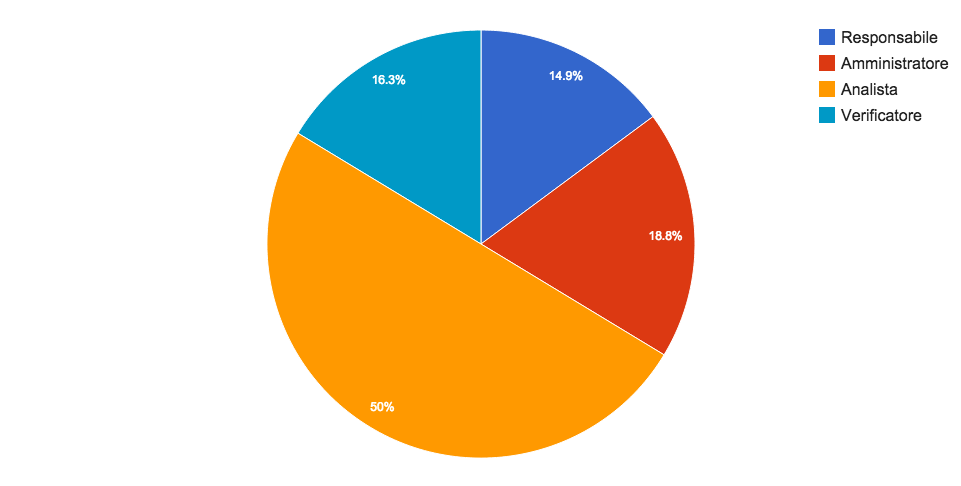
\includegraphics[width=0.4\textwidth]{../immagini/nuoviGrafici/oreFaseAnalisi.png}% "%" necessario
%\qquad\qquad
%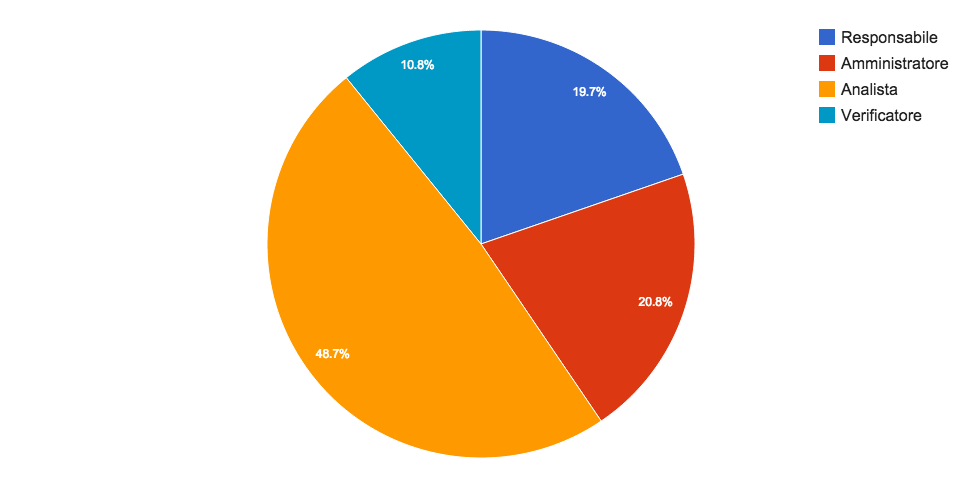
\includegraphics[width=0.4\textwidth]{../immagini/nuoviGrafici/costoFaseAnalisi.png}
%\caption{Divisione delle ore e dei costi - Fase di \fAt}
%\end{figure}
% \FloatBarrier
\subsubsection{Fase di \fADt}
\subsubsubsection{Suddivisione del lavoro}
Nella fase di \fAD, ciascun componente dovrà rivestire i seguenti ruoli:
%tabella suddivisione
\begin{table}[h]
\begin{center}
\begin{tabular}{|c|c|c|c|c|c|c|c|}
\hline Nome & Re & Am & An & Pt & Pr & Ve & Ore totali\\
\hline
\gma & - & - & 4 & - & - & 2 & 6 \\
\ao & 6 & - & - & - & - & - & 6 \\
\mb & - & - & - & - & - & 5 & 5 \\
\dm & - & - & 6 & - & - & - & 6 \\
\gmi & - & 5 & - & - & - & 3 & 8 \\
\sm & - & - & 4 & - & - & 3 & 7 \\
\fv & - & - & 5 & - & - & 1 & 6 \\
\hline Totale ruoli & 6 & 5 & 19 & - & - & 14 & 44 \\
\hline
\end{tabular}
\caption{Ore per ruolo - Fase di \fADt}
\end{center}
\end{table}
\FloatBarrier
I valori vengono riassunti nel seguente grafico:
\begin{figure}[htbp]
\centering
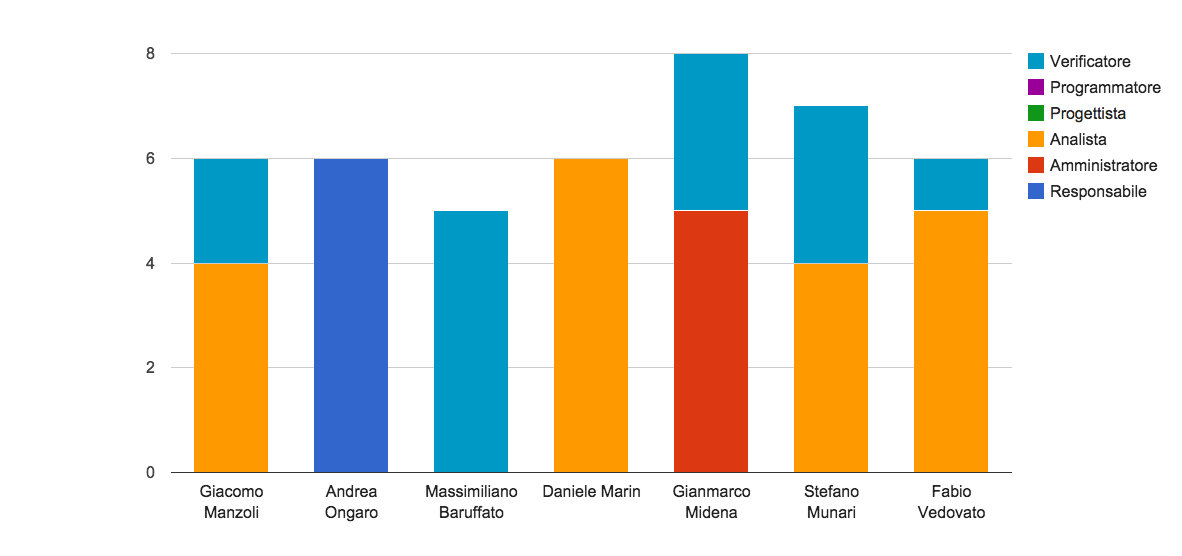
\includegraphics[width=\textwidth]{../immagini/nuoviGrafici/componenti/oreCompFaseAnalisiDet.png}
\caption{Ore per componente - Fase di \fADt}
\end{figure}
\FloatBarrier
\subsubsubsection{Prospetto economico}
Il totale delle ore di lavoro di ogni ruolo e il relativo costo \uline{a carico del \gloxy{fornitore}} vengono riportati nella seguente tabella:
\begin{table}[h]
\begin{center}
\begin{tabular}{|m{3cm}|m{1.5cm}|m{1.5cm}|}
\hline Ruolo & Ore & Costo (\euro) \\
\hline
\rRPt & 6 & 180 \\
\rAPt & 5 & 125 \\
\rAt & 19 & 418 \\
\rPt & 0 & 0 \\
\rpt & 0 & 0 \\
\rVt & 14 & 210 \\
\hline
Totale & 44 & 933 \\
\hline
\end{tabular}
\caption{Prospetto economico - Fase di \fADt}
\end{center}
\end{table}
\FloatBarrier
I seguenti grafici illustrano rispettivamente come ciascun ruolo abbia influito sul totale delle ore e dei costi \uline{a carico del \gloxy{fornitore}} durante la fase di \fAD.
\begin{figure}[h]
\centering
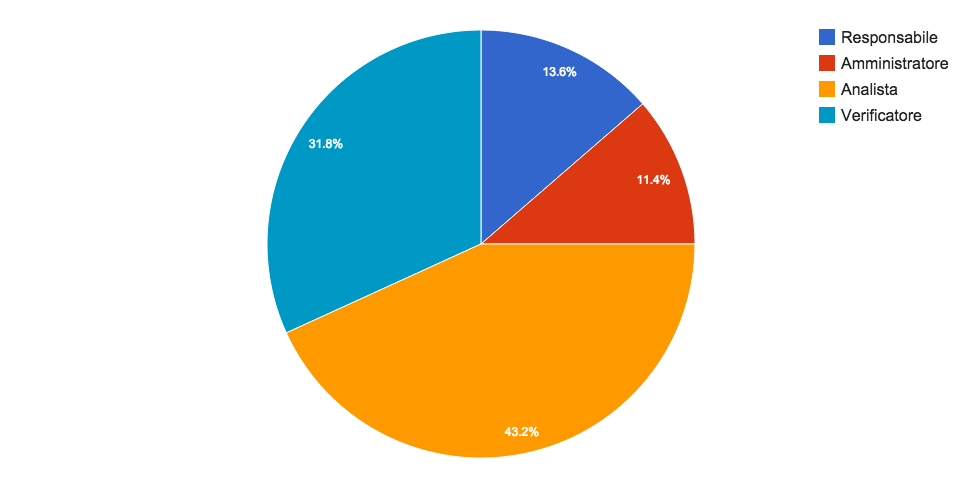
\includegraphics[width=0.9\textwidth]{../immagini/nuoviGrafici/oreFaseAnalisiDet.png}
\caption{Ore per ruoli - Fase di \fADt}
\end{figure}
\begin{figure}[h]
\centering
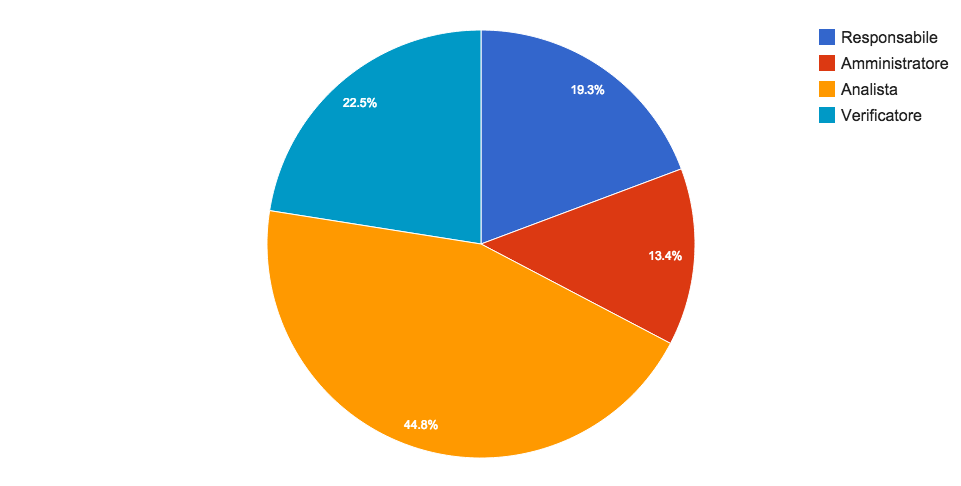
\includegraphics[width=0.9\textwidth]{../immagini/nuoviGrafici/costoFaseAnalisiDet.png}
\caption{Costi per ruoli - Fase di \fADt}
\end{figure}
\FloatBarrier
%-----------------------------------------------------------------
\subsection{Totali considerando l'investimento}
\subsubsection{Suddivisione del lavoro}
Le ore totali, comprese quelle di investimento, che ogni componente dedicherà ad un determinato ruolo sono espresse nella seguente tabella:
%tabella suddivisione
\begin{table}[h]
\begin{center}
\begin{tabular}{|c|c|c|c|c|c|c|c|}
\hline Nome & Re & Am & An & Pt & Pr & Ve & Ore totali\\
\hline
\gma & 18 & 12 & 6 & 41 & 23 & 40 & 140 \\
\ao & 6 & 8 & 26 & 49 & 35 & 16 & 140 \\
\mb & 3 & 18 & 17 & 49 & 23 & 29 & 139 \\
\dm & 13 & 4 & 18 & 49 & 23 & 31 & 138 \\
\gmi & 8 & 5 & 26 & 34 & 5 & 61 & 139 \\
\sm & 3 & 8 & 27 & 49 & 12 & 40 & 139 \\
\fv & 6 & 8 & 25 & 34 & 11 & 55 & 139 \\
\hline Totale ruoli & 57 & 63 & 145 & 305 & 132 & 272 & 974 \\
\hline
\end{tabular}
\caption{Ore per ruolo - Totali, comprese le ore di investimento}
\end{center}
\end{table}
\FloatBarrier
I valori vengono riassunti nel seguente grafico:
\begin{figure}[htbp]
\centering
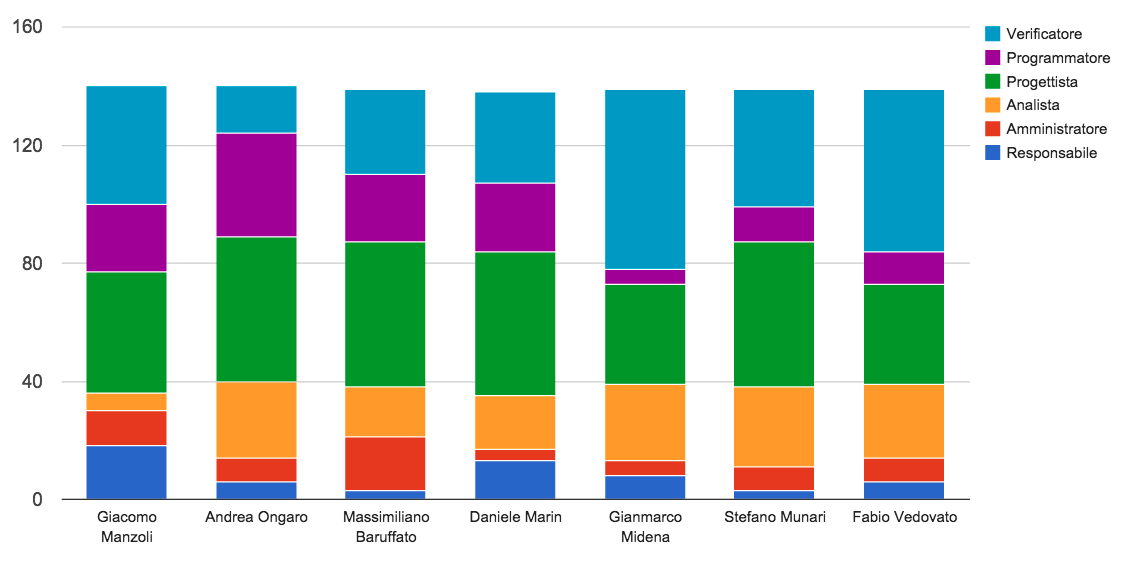
\includegraphics[width=\textwidth]{../immagini/nuoviGrafici/componenti/oreCompTotaliInvestimento.png}
\caption{Ore per componente - Totali, comprese le ore di investimento}
\end{figure}
\FloatBarrier
\subsubsection{Prospetto economico}
Le ore totali, comprese quelle di investimento, previste per la realizzazione del \gloxy{progetto} sono riportate nella seguente tabella:
\begin{table}[h]
\begin{center}
\begin{tabular}{|m{3cm}|m{1.5cm}|m{1.5cm}|}
\hline Ruolo & Ore & Costo (\euro) \\
\hline
\rRPt & 57 & 2070 \\
\rAPt & 63 & 1700 \\
\rAt & 145 & 3190 \\
\rPt & 305 & 6480 \\
\rpt & 132 & 1995 \\
\rVt & 272 & 3765 \\
\hline
Totale & 974 & 18635 \\
\hline
\end{tabular}
\caption{Prospetto economico - Totale, comprese le ore di investimento}
\end{center}
\end{table}
\FloatBarrier
I seguenti grafici illustrano rispettivamente come ciascun ruolo abbia influito sul totale delle ore e dei costi del \gloxy{progetto}.
%grafico a torta dei costi e delle ore
\begin{figure}[h]
\centering
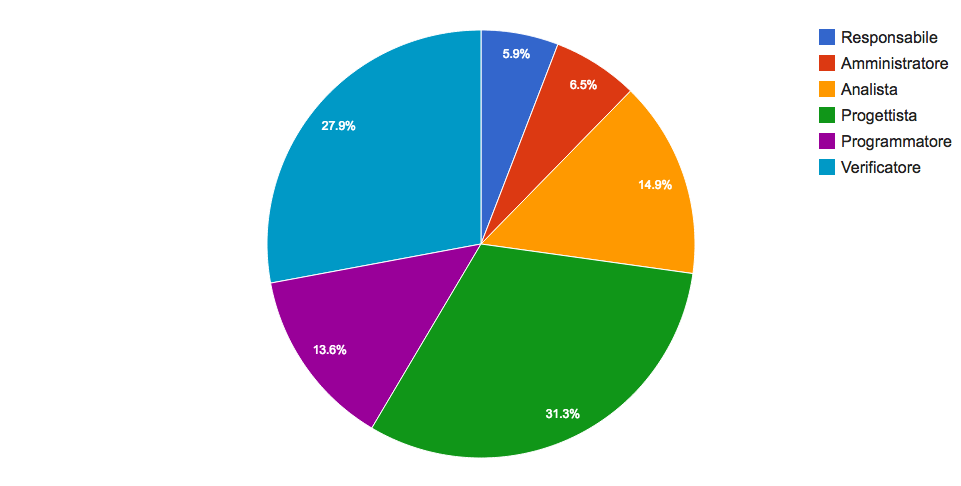
\includegraphics[width=0.9\textwidth]{../immagini/nuoviGrafici/oreTotaliConAnalisi.png}
\caption{Ore per ruoli - Totali, con investimento}
\end{figure}
\begin{figure}[h]
\centering
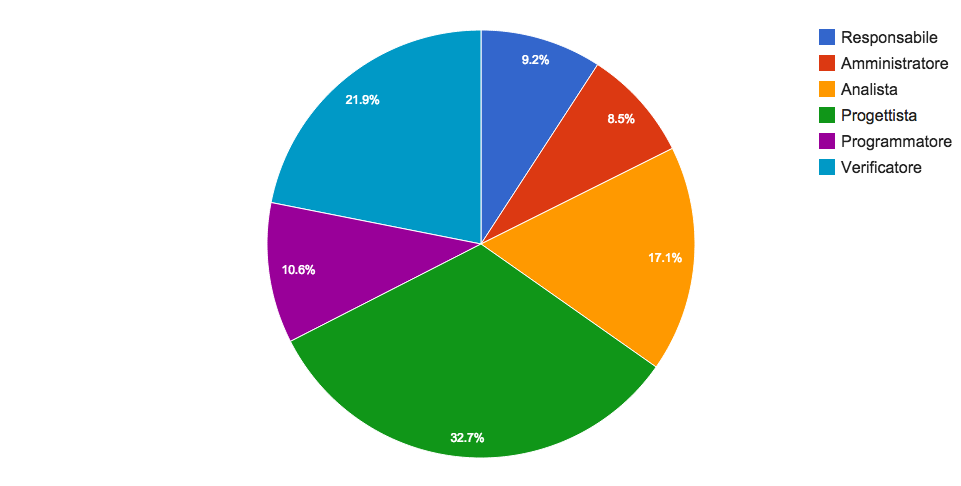
\includegraphics[width=0.9\textwidth]{../immagini/nuoviGrafici/costoTotaleConAnalisi.png}
\caption{Costi per ruoli - Totali, con investimento}
\end{figure}
\FloatBarrier
